
%============================================================
\subsection{\texttt{notched\_cylinder}}
\label{subsec:geometry_notched_cylinder}
%============================================================

\noindent
\textbf{Geometry ID:} \texttt{GLOB-GEO0007}
\qquad
\textbf{Version:} \texttt{1.0.0}

\begin{figure}[htbp]
    \centering
    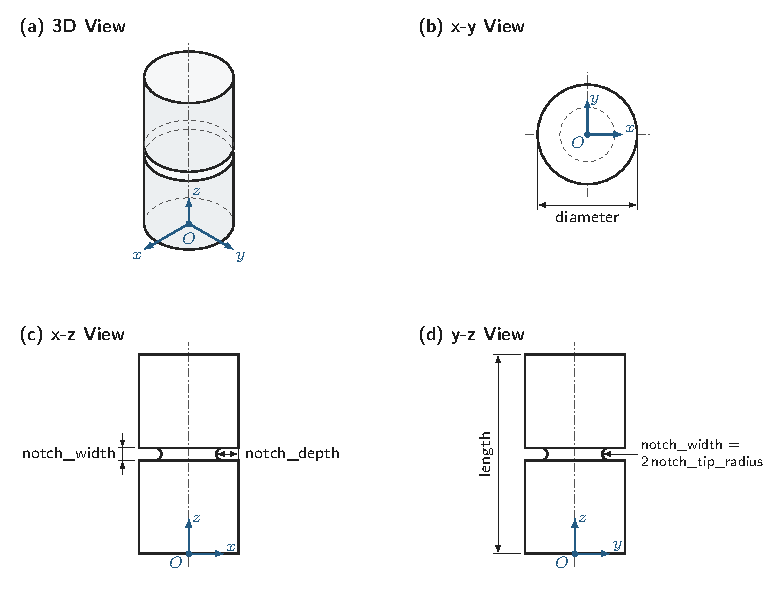
\includegraphics[width=0.65\linewidth]
    {./figs/geometries/notched_cylinder.pdf}
    \caption{Standardized parametrization and local
    coordinate system of the notched cylinder geometry.}
    \label{fig:notched_cylinder}
\end{figure}

The \texttt{notched\_cylinder} geometry represents
a right circular cylindrical specimen containing
an axisymmetric circumferential notch centered
at longitudinal midspan.

As illustrated in Fig.~\ref{fig:notched_cylinder},
the local coordinate system is defined by
the right-handed Cartesian axes $x$, $y$,
and $z$. The origin $O$ is located at
the center of the reference circular end face,
corresponding to $z=0$.

The $z$ axis coincides with the longitudinal
axis of the cylinder, while the $x$ and $y$
axes define the transverse plane.

The circumferential notch is centered at

\begin{equation}
z=\frac{\texttt{length}}{2}.
\end{equation}

In an axial section, the notch has parallel
sides terminating in a semicircular tip.

\paragraph{Independent parameters.}

The geometry is defined by four required
parameters, all expressed in millimeters:

\begin{itemize}
    \item \texttt{length}: cylinder length
    measured along the local $z$ axis;

    \item \texttt{diameter}: outer cylinder
    diameter measured in the local
    $x$--$y$ plane;

    \item \texttt{notch\_depth}: total radial
    penetration measured inward from the
    original cylindrical surface to the
    deepest point of the semicircular tip;

    \item \texttt{notch\_width}: axial opening
    width of the circumferential notch,
    measured along the local $z$ axis.
\end{itemize}

\paragraph{Derived parameters.}

The notch terminates in a semicircular tip
whose radius is determined by

\begin{equation}
\texttt{notch\_tip\_radius}
=\frac{\texttt{notch\_width}}{2}.
\end{equation}

The radius is therefore a derived quantity
and is not an independent input parameter.

\paragraph{Geometric constraints.}

All independent parameters must be strictly
positive. The notch geometry must additionally
satisfy

\begin{align}
\texttt{notch\_depth}
&< \frac{\texttt{diameter}}{2},
\\
\texttt{notch\_width}
&< \texttt{length},
\\
\texttt{notch\_depth}
&> \frac{\texttt{notch\_width}}{2}.
\end{align}

The first condition ensures a strictly positive
remaining radius at the notch root. The second
ensures that the notch remains within the
longitudinal extent of the cylinder. The third
requires a strictly positive straight-sided
radial portion preceding the semicircular tip.
